\documentclass[11pt]{article}
\usepackage[margin=1in]{geometry}
\usepackage{graphicx}
\usepackage{booktabs}
\usepackage{amsmath}
\usepackage{amssymb}
\usepackage{hyperref}
\usepackage{natbib}
\usepackage{caption}
\usepackage{float}

\title{Predicted Gene-Program Activations from Histology Are Fragile to Routine Image Perturbations, and the Failure Mode Depends on the Encoder}
\author{Abdelrahman A. Alshames$^{*}$\\[4pt]
\small Faculty of Computer Science and Information Technology,\\
\small Egypt-Japan University of Science and Technology (E-JUST), New Borg El Arab, Alexandria, Egypt\\[4pt]
\small $^{*}$Corresponding author: \texttt{abdelrahman.aboegela@ejust.edu.eg}}
\date{\today}

\begin{document}
\maketitle

\begin{abstract}
Virtual spatial transcriptomics -- predicting gene expression from H\&E histology via frozen pathology foundation models -- is increasingly used to derive biomarkers for treatment decisions. We ask whether the gene-program activations these pipelines produce are stable under routine clinical image variation: JPEG compression, brightness/contrast/gamma shift, blur, scanner color shift, and H\&E stain variation. Using two frozen encoders (CONCH, UNI) with a linear probe on two independent Xenium cohorts from HEST-Bench (breast IDC, colorectal COAD), and after removing a library-size confound, we confirm real predictive signal on both cohorts, clearing two floor baselines and partially corroborated by a leave-one-slide-out check. We introduce a Gene-Program Flip Rate (GPFR), an instantiation of the decision-flip-rate family of instability metrics applied to continuous Hallmark-aggregated program scores, statistically distinguishable from a boundary null for most perturbation-program combinations under a slide-level cluster bootstrap. CONCH's dominant failure mode, scanner-color shift, replicates cleanly across both cohorts and all eight re-splits; UNI's is JPEG compression on IDC but a near-tie among three perturbations on COAD. This is direct evidence that a fragility profile measured on one encoder, and on one cohort, does not safely generalize to another, with consequences for how virtual spatial-transcriptomics robustness should be evaluated and reported.
\end{abstract}

\noindent\textbf{Keywords:} virtual spatial transcriptomics; computational pathology; foundation models; robustness; digital pathology; gene-program prediction

\section{Introduction}

Predicting spatial gene expression directly from H\&E histology images -- ``virtual spatial transcriptomics'' -- has moved from a methods-only exercise to a component of real clinical-translation pipelines. \citet{nature_medicine_2025_virtual_st} deployed a virtual spatial-proteomics pipeline across 2{,}298 non-small-cell lung cancer patients and reported a 24--39\% improvement in immunotherapy response prediction. As these predicted biomarkers move closer to influencing treatment decisions, a natural question follows: how stable are they under the image variation that occurs routinely, and without any adversarial intent, in real deployment?

Two forms of routine variation are well documented and unavoidable at multi-site scale. JPEG compression is standard practice for whole-slide-image storage and transfer -- \citet{jpeg_compression_pathology} note it remains the majority WSI vendor practice, and the DICOM WSI standard \citep{dicom_wsi_standard} states pathologists have found no loss of diagnostic information at compression ratios of 15--20$\times$; this is the regime we use to anchor our perturbation magnitudes (Section~\ref{sec:methods}). H\&E stain appearance varies substantially across labs, scanners, and reagent batches; \citet{plism_protocol} formalize this with a 46-tissue $\times$ 13-condition $\times$ 7-scanner reference protocol.

A closely related benchmarking effort, \citet{wang2025_translational}, found that at least one gene-expression-prediction method's accuracy correlates with naturally-occurring image quality variation in TCGA slides (Pearson $r=0.53$ for one method, near-zero for two others) -- independent evidence that this concern is real. That study's robustness measurement is, however, \emph{correlational} (natural quality variation regressed against accuracy) and entirely \emph{gene-level}. We ask a different, complementary question: under a \emph{controlled}, \emph{calibrated} perturbation applied to the same image, does the \emph{program-level} (Hallmark-aggregated) prediction -- the level at which these outputs are actually interpreted biologically -- flip categorically, and does that answer depend on which frozen foundation-model encoder is used underneath.

\citet{stpbench_2026} note that architecture effects have been conflated with encoder effects across this subfield, and that ``evaluation has been confined to aggregate predictive accuracy, leaving the biological reliability of virtual ST and model robustness under realistic distribution shifts largely unexamined.'' \citet{wang2025_translational} benchmarked eleven histology-to-expression methods and explicitly tested ``robustness to input quality,'' the closest existing work to this paper; their measurement is correlational and gene-level, using the older end-to-end CNN/ViT architectures (DeepPT, HisToGene, Hist2ST) rather than the modern frozen-foundation-model-plus-linear-probe paradigm we use here. \citet{stimage_2026} also use the word ``robust,'' but to mean cross-cohort and cross-platform generalization plus aleatoric/epistemic uncertainty quantification via encoder ensembling -- a different question from perturbation-induced instability -- and \citet{utopia_2026} measures calibrated confidence rather than perturbation-induced flip behavior. \citet{utap_2026} address a different threat model entirely, introducing a universal, transferable, gradient-optimized adversarial perturbation against seven pathology foundation models; that is a security question (can an adversary degrade the model), distinct from ours (does routine, non-adversarial clinical variation degrade the model). \citet{pathorob_2026} found robustness deficits across all 20 foundation models they evaluated on standard (non-expression) tasks, and \citet{robustifying_fms_2607} found that scanner-shift is approximately linear in pathology-FM feature space across 10 models; both motivate our mechanistic decomposition (Section~\ref{sec:fragility_decomposition}) rather than treating GPFR as a black-box number. \citet{crossplatform_st_het} document off-target probe binding and large panel-size differences (targeted $\sim$300 genes vs.\ whole-transcriptome $\sim$20--36k genes) across spatial platforms, relevant to our decision to restrict the analysis to a single platform (Xenium, across two organs) rather than pool across the platform boundary. \citet{pearl_2510} (PEaRL) and \citet{histoprism_2026} (HistoPrism) are the closest architectural neighbors for pathway-level prediction from histology; both are accuracy contributions rather than robustness ones, and neither uses a frozen-encoder-plus-linear-probe architecture, so they answer a different question (does architecture, not just encoder, change the failure mode) than the one this paper asks.

\textbf{Contributions.} (1) We instantiate a Gene-Program Flip Rate (GPFR) metric for program-level instability under calibrated, morphology-preserving perturbations, with a slide-level cluster bootstrap for confidence intervals and FDR-corrected significance testing. (2) We show, on identical data and task and stable across four independent train/held-out re-splits, that CONCH and UNI have genuinely different dominant failure modes (scanner-color shift vs.\ JPEG compression) whose four-seed magnitude ranges do not overlap in either direction. (3) We identify and control for a library-size/cellularity confound in the modeling target that a naive fit would substantially exploit instead of learning gene-program biology, validating the correction against two floor baselines and a dedicated diagnostic script rather than by assertion alone. (4) We report a spatially-disjoint (leave-one-slide-out) validity check showing that the conventional random-split validity number is inflated relative to a genuinely unseen slide -- a check this kind of study should run and typically does not. (5) We repeat the full analysis on a second, independently downloaded organ (COAD) on the same platform, and find CONCH's dominant failure mode replicates cleanly while UNI's does not, itself informative about which parts of an encoder's fragility profile can be expected to transfer across cohorts.

\section{Results}
\label{sec:results}

\subsection{Predictive validity}
Table~\ref{tab:validity} reports held-out predictive validity for both encoders under a random 70/30 patch split. CONCH: $r=0.559$ (whole panel), $0.614$ (Hallmark genes); UNI: $r=0.604$, $0.661$. The Hallmark-restricted $r$ exceeding the whole-panel $r$ for both encoders indicates the per-target-$\alpha$ Ridge fitting (Section~\ref{sec:methods}) is working where it matters: the whole-panel mean is dragged down by many genes on this 280-gene targeted panel with little real histological signal, which is expected biology rather than a modeling failure. Section~\ref{sec:loso} reports a further, spatially-disjoint check on this number, since the random patch split used here cannot rule out train/held-out pixel overlap.

\begin{table}[t]
\centering
\caption{Held-out (out-of-sample) predictive validity on IDC and COAD (2100 train / 900 held-out patches per organ, seed=42). Ridge $\alpha$ selected per-gene via efficient leave-one-out cross-validation (\texttt{RidgeCV}, \texttt{alpha\_per\_target=True}); median [min, max] shown across the panel's genes.}
\label{tab:validity}
\begin{tabular}{llccc}
\toprule
Organ & Encoder & $r$ (whole panel) & $r$ (Hallmark genes) & Ridge $\alpha$ \\
\midrule
IDC & CONCH (ViT-B/16, 86M) & 0.559 & 0.615 & 100 [3.16, 3.16e+04] \\
IDC & UNI (ViT-L/16, 307M) & 0.605 & 0.662 & 3.16e+03 [316, 3.16e+04] \\
COAD & CONCH (ViT-B/16, 86M) & 0.604 & 0.697 & 100 [10, 1e+05] \\
COAD & UNI (ViT-L/16, 307M) & 0.650 & 0.742 & 1e+03 [316, 1e+05] \\
\bottomrule
\end{tabular}
\end{table}


\subsection{Predictive validity clears two floor baselines}
\label{sec:baselines}
Pearson $r$ alone does not establish that a model uses the histology image meaningfully. Table~\ref{tab:baseline_comparison} reports held-out $R^2$ -- the metric that remains well-defined for a constant-prediction baseline -- for CONCH-Ridge and UNI-Ridge against \texttt{training-mean} (no image at all) and \texttt{total-counts-linear} (one feature: the patch's own raw, pre-normalization total transcript count, i.e.\ the confound the library-size normalization step, Section~\ref{sec:methods}, removes from the modeling target). Both real models clear both floors by a wide margin ($R^2=0.339$/$0.391$ whole-panel, $0.402$/$0.463$ Hallmark-restricted, for CONCH/UNI respectively) against \texttt{training-mean}'s $R^2\approx0$ and \texttt{total-counts-linear}'s $R^2\approx0.07$. The latter number bears a specific interpretation: after per-patch normalization, every patch's target sums to exactly the cohort median by construction, so a raw-count feature cannot recover the target's overall \emph{scale} regardless of any confound -- this baseline can only detect whether raw cellularity still covaries with \emph{relative} gene composition. Its small but nonzero $R^2\approx0.07$ is consistent with normalization removing most, though not all, of that confound from relative composition.

\begin{table}[t]
\centering
\caption{Held-out $R^2$ against two floor baselines, identical IDC and COAD train/held-out splits as Table~\ref{tab:validity} (seed=42). \texttt{Training-mean} predicts every held-out patch with the training set's per-gene mean (no image, no metadata). \texttt{Total-counts-linear} predicts from a single feature -- the patch's own raw (pre-normalization) total panel counts -- exactly the confound the library-size normalization fix targets; because normalization makes every patch's target sum to the same value by construction, this baseline can only detect a confound in \emph{relative} composition, not overall scale, so its small $R^2$ is a limited, not fully independent, check.}
\label{tab:baseline_comparison}
\begin{tabular}{llcc}
\toprule
Organ & Model & $R^2$ (whole panel) & $R^2$ (Hallmark genes) \\
\midrule
IDC & CONCH-Ridge (ours) & 0.339 & 0.402 \\
IDC & UNI-Ridge (ours) & 0.391 & 0.463 \\
IDC & Training-mean (no image) & -0.002 & -0.001 \\
IDC & Total-counts-linear (1 feature) & 0.068 & 0.070 \\
COAD & CONCH-Ridge (ours) & 0.400 & 0.495 \\
COAD & UNI-Ridge (ours) & 0.459 & 0.562 \\
COAD & Training-mean (no image) & -0.002 & -0.002 \\
COAD & Total-counts-linear (1 feature) & 0.080 & 0.122 \\
\bottomrule
\end{tabular}
\end{table}


\subsection{Spatially-disjoint validity: real signal, but limited absolute-scale transfer across slides}
\label{sec:loso}
A random patch split cannot rule out two sources of optimism in the reported $r$/$R^2$: ordinary spatial autocorrelation in Xenium expression, and direct pixel overlap between train and held-out patches. On IDC, the patch extraction size exceeds the tiling grid pitch on every sample (e.g.\ sample NCBI783: 409\,px patches on a 365\,px grid, a 44\,px/$\sim$11\% overlap band along each shared edge); adjacent patches' shared border pixels are highly correlated ($r=0.99$), confirming genuine pixel overlap rather than a nominal grid artifact. Under a random 70/30 split, 49.1\% of held-out patches share some physical pixel overlap with at least one training patch (32.0\% share a full edge), unevenly across slides -- from 77.4\% on NCBI783 down to 13.7\% on TENX99, tracking each slide's patch-to-pitch ratio.

We therefore also ran a 4-fold leave-one-slide-out check: for each of IDC's 4 slides in turn, the Ridge head is fit on the other 3 slides' patches entirely and evaluated on the held-out slide, which by construction shares no patches, no pixels, and no local spatial structure with the training set. This is also leave-one-\emph{patient}-out, not merely leave-one-slide-out: HEST-Bench's metadata lists IDC's 4 samples as 4 distinct patients, so no fold's evaluation slide is a serial section of, or otherwise related to, its training slides. Held-out Pearson $r$ remains clearly positive but is lower than the random-split number: CONCH $r=0.337$ (whole panel, range across the 4 held-out slides $0.254$--$0.405$), $0.428$ Hallmark-restricted ($0.329$--$0.512$); UNI $r=0.360$ ($0.274$--$0.415$), $0.459$ Hallmark-restricted ($0.360$--$0.534$). The model therefore captures real, slide-transferable rank information about gene-program activation from histology, rather than an artifact of the pixel overlap described above.

Held-out $R^2$ under this same check is a more complex picture than $r$. The \emph{mean} per-gene $R^2$ (scikit-learn's default multi-output average) is strongly negative for both encoders (CONCH: whole-panel $-19.8$, range $-68.9$ to $-1.05$; Hallmark-restricted $-0.65$, range $-1.29$ to $-0.42$; UNI: whole-panel $-9.0$, range $-25.2$ to $-0.84$; Hallmark-restricted $-0.46$, range $-0.70$ to $-0.30$). Because $R^2$ is unbounded below, a handful of genes with a large between-slide mean offset relative to their within-slide variance dominate that mean -- on the CONCH/NCBI785 fold, for example, a mean whole-panel $R^2=-68.9$ corresponds to a \emph{median} per-gene $R^2$ of only $-0.24$. Table~\ref{tab:loso_validity} reports both statistics: the median-of-per-fold-medians whole-panel $R^2$ is $-0.14$ (CONCH) and $-0.07$ (UNI); Hallmark-restricted, it is $-0.005$ (CONCH, essentially break-even) and $+0.065$ (UNI). A negative $R^2$ here means the model performs worse than an oracle that already knows the held-out slide's own true per-gene mean -- a strictly harder bar than the training-mean baseline in Table~\ref{tab:baseline_comparison} clears, since that baseline is evaluated against the training set's mean instead. In summary, the median gene's out-of-slide calibration is close to break-even, while a real subset of genes calibrate poorly in absolute terms across slides, plausibly reflecting an unmodeled Xenium batch effect in absolute expression scale that per-patch library-size normalization does not correct for.

\begin{table}[t]
\centering
\caption{Leave-one-slide-out validity on IDC: Ridge head fit on 3 slides, evaluated on the 4th (never seen during fitting), for every slide in turn. Compare $r$ against Table~\ref{tab:validity}'s random-split numbers (CONCH 0.559/0.614, UNI 0.604/0.661 whole-panel/Hallmark) -- lower here, but still clearly positive. $R^2$(mean) is the standard multi-output average across genes; $R^2$(median) is the median per-gene value, reported because a handful of outlier genes with poor between-slide calibration dominate the mean (e.g.\ CONCH/NCBI785: mean $-68.9$, median $-0.24$) -- the median is a better summary of the typical gene's out-of-slide calibration, though both are real and disclosed here rather than only the more dramatic one. The bottom row of each encoder block is that encoder's mean $r$/mean $R^2$ across its 4 folds, with the median column showing the median of each fold's own per-gene median (not re-derived from pooled per-gene values).}
\label{tab:loso_validity}
\resizebox{\textwidth}{!}{%
\begin{tabular}{llcccccc}
\toprule
Encoder & Held-out slide & $r$ & $r$ (Hallmark) & $R^2$ (mean) & $R^2$ (median) & $R^2_{\text{Hallmark}}$ (mean) & $R^2_{\text{Hallmark}}$ (median) \\
\midrule
CONCH & NCBI783 & 0.302 & 0.389 & -1.14 & -0.031 & -0.45 & -0.002 \\
CONCH & NCBI785 & 0.387 & 0.484 & -68.88 & -0.241 & -0.42 & -0.008 \\
CONCH & TENX95 & 0.405 & 0.512 & -1.05 & -0.152 & -0.42 & 0.018 \\
CONCH & TENX99 & 0.255 & 0.329 & -8.25 & -0.126 & -1.29 & -0.107 \\
\textit{CONCH mean} & -- & 0.337 & 0.428 & -19.83 & -0.139 & -0.65 & -0.005 \\
UNI & NCBI783 & 0.337 & 0.425 & -0.84 & 0.000 & -0.30 & 0.079 \\
UNI & NCBI785 & 0.414 & 0.519 & -25.19 & -0.093 & -0.38 & 0.084 \\
UNI & TENX95 & 0.415 & 0.534 & -1.07 & -0.069 & -0.44 & 0.050 \\
UNI & TENX99 & 0.274 & 0.360 & -8.71 & -0.072 & -0.70 & -0.039 \\
\textit{UNI mean} & -- & 0.360 & 0.459 & -8.96 & -0.070 & -0.46 & 0.065 \\
\bottomrule
\end{tabular}%
}
\end{table}


\subsection{GPFR is statistically significant, and the failure mode is encoder-dependent}
Figure~\ref{fig:gpfr_divergence} plots peak GPFR per perturbation for both encoders on IDC; Section~\ref{sec:coad_generalization} repeats this analysis on a second, independent organ. Supplementary Tables~S1 and S2 report GPFR for all 35 (perturbation, program) combinations per encoder, with 95\% CIs from the slide-level cluster bootstrap (Section~\ref{sec:methods}). A combination is starred when it clears FDR$<$0.05 \emph{and} its CI excludes 0.000 (Section~\ref{sec:methods}); \textbf{34/35} combinations meet this bar for CONCH (only \texttt{gamma}/\texttt{immune\_activation}, GPFR$=0.003$, does not, $q=0.065$) and \textbf{31/35} for UNI (\texttt{blur}/\texttt{immune\_activation}, \texttt{stain\_shift}/\texttt{immune\_activation}, \texttt{blur}/\texttt{proliferation}, and \texttt{blur}/\texttt{stromal\_ecm} do not). \emph{Significant} here means \emph{distinguishable from exactly zero} given the sample size and slide count, not \emph{large}; Supplementary Tables~S1--S2's point estimates and CI widths, not the significance stars, indicate magnitude and precision (see Section~\ref{sec:limitations} for the CI-width caveat).

The two encoders do not agree on which perturbation matters most. CONCH's largest effect is \texttt{scanner\_color} (hypoxia GPFR$=0.399$), well clear of its next-largest (\texttt{brightness}/hypoxia and \texttt{scanner\_color}/immune\_activation, both $0.191$); UNI's largest effect is \texttt{jpeg} (immune\_activation GPFR$=0.264$), the single largest GPFR either encoder produced, with UNI's \texttt{blur} its weakest perturbation across every program ($\le 0.022$). Section~\ref{sec:seed_stability} checks whether this ranking survives a different train/held-out split.

\begin{figure}[t]
\centering
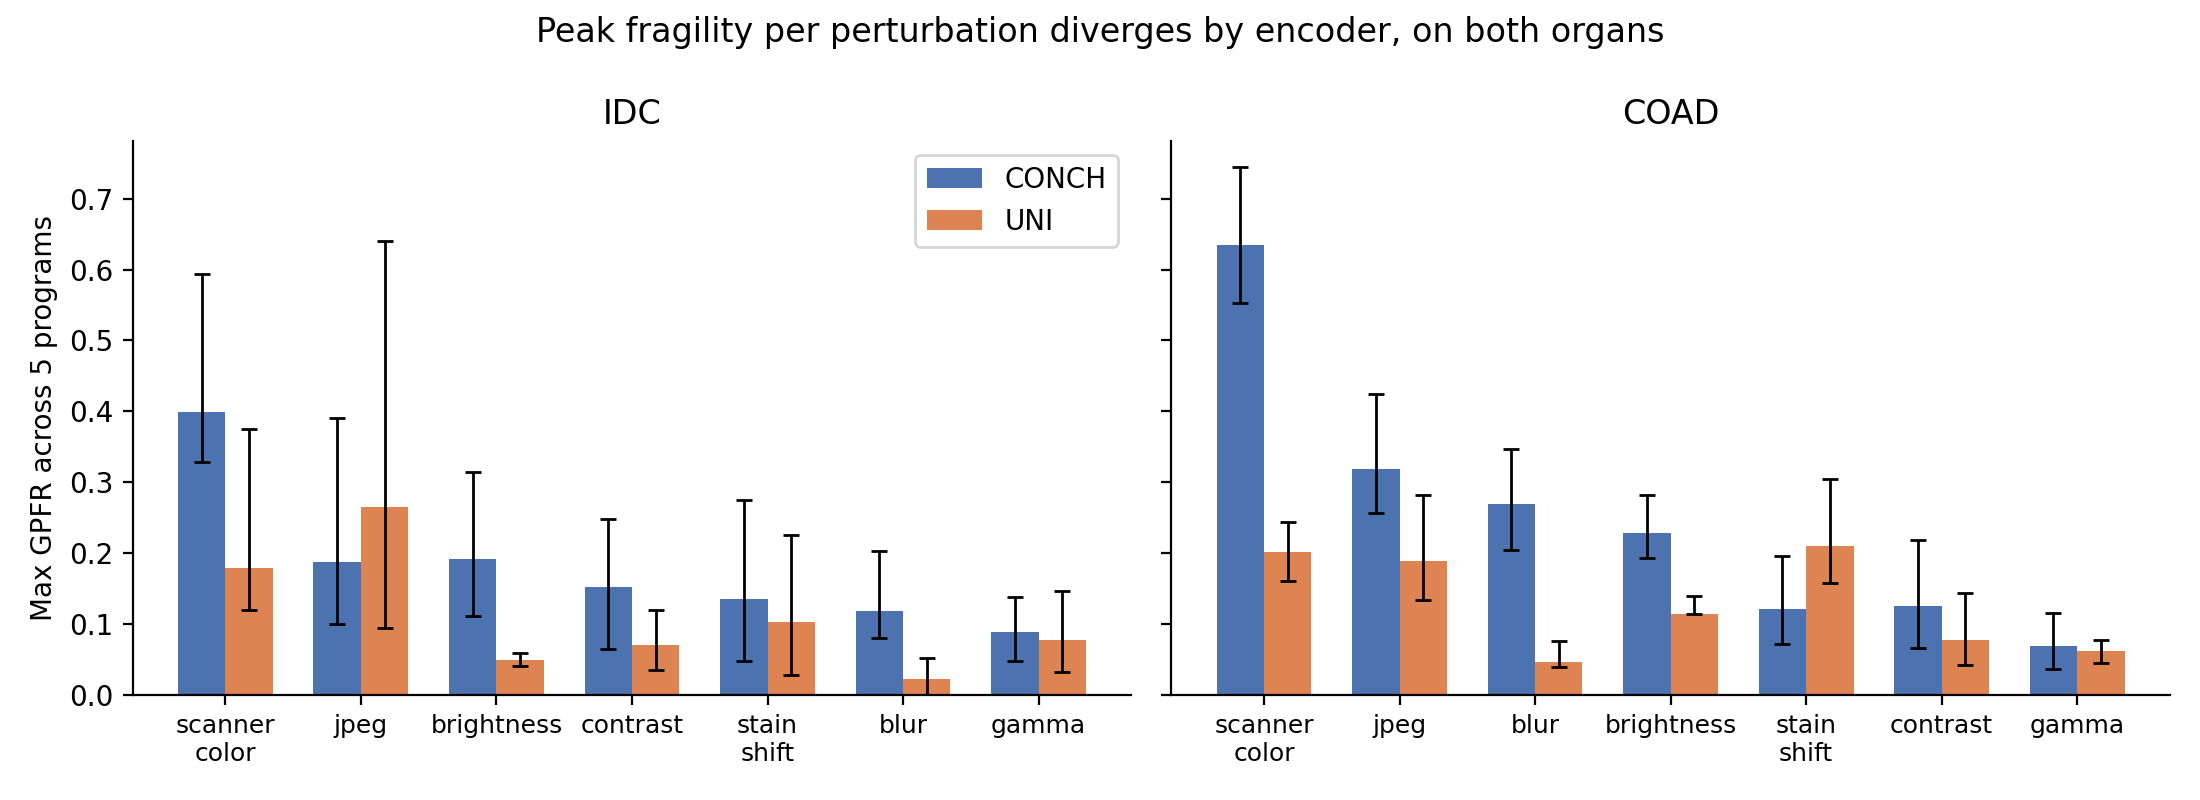
\includegraphics[width=0.8\textwidth]{figures/gpfr_encoder_divergence.png}
\caption{Peak GPFR (maximum across the 5 Hallmark programs) per perturbation, for both encoders on IDC and COAD (seed 42). \texttt{scanner\_color} is CONCH's dominant failure mode on both organs. UNI's dominant mode is \texttt{jpeg} on IDC but a near-tie among \texttt{stain\_shift}, \texttt{jpeg}, and \texttt{scanner\_color} on COAD (Section~\ref{sec:coad_generalization}). Section~\ref{sec:seed_stability} shows CONCH's IDC ranking is stable across four independent train/held-out splits, and that each encoder's dominant perturbation's range does not overlap the other encoder's range for that same perturbation. Error bars are 95\% bootstrap CIs.}
\label{fig:gpfr_divergence}
\end{figure}

\subsection{Stability of the ranking across independent train/held-out splits}
\label{sec:seed_stability}
The analysis above uses one random 70/30 split (seed 42); we repeat it for both encoders at three additional seeds (7, 123, 2024). Tables~\ref{tab:seed_stability} and \ref{tab:seed_stability_uni} report the result: for both encoders, one perturbation has the highest mean max-GPFR at every one of the 4 splits. CONCH's \texttt{scanner\_color} (mean max-GPFR $0.367\pm0.051$, range $0.293$--$0.406$) leads the next-highest perturbation by at least $0.10$ at every seed. UNI's \texttt{jpeg} (mean max-GPFR $0.253\pm0.016$) leads by a smaller and less uniform margin ($0.081$--$0.144$ across the 4 seeds). \texttt{blur} is UNI's most stable perturbation by standard deviation ($0.006$) and its weakest by mean ($0.019\pm0.006$, range $0.010$--$0.022$).

A cross-encoder magnitude comparison is not automatically scale-free, because GPFR's denominator is each encoder's own cohort standard deviation. Recomputing max-GPFR at seed 42 against a single pooled (encoder-independent) $\sigma_c$ per program instead of each encoder's own, the \texttt{jpeg} gap (UNI max $-$ CONCH max) narrows from $0.078$ (own $\sigma_c$) to $0.051$ (pooled $\sigma_c$) but remains positive and substantial; \texttt{scanner\_color}'s gap (already favoring CONCH) does not narrow under pooling ($-0.220$ to $-0.249$). The direction of the divergence therefore survives a shared scale for both perturbations, and the cross-encoder divergence claim rests on this pooled-cohort, multi-seed result: the two encoders' four-seed ranges for each other's dominant perturbation do not overlap. UNI's \texttt{jpeg} range ($0.233$--$0.268$) is entirely above CONCH's four-seed \texttt{jpeg} range ($0.110$--$0.187$); CONCH's \texttt{scanner\_color} range ($0.293$--$0.406$) is entirely above UNI's four-seed \texttt{scanner\_color} range ($0.091$--$0.187$).

A seed re-split resamples the same 4 slides rather than drawing new ones, so it cannot distinguish ``dominant for this model'' from ``dominant because of how these particular 4 slides are weighted.'' We therefore also computed max-GPFR restricted to each individual slide, using each slide's own within-slide $\sigma_c$. This breakdown has two limitations. First, the 5 calibrated perturbations share one magnitude across the whole IDC cohort, but the slides differ in patch-extraction resolution by up to $1.7\times$, so delivered dose (in SSIM terms) varies substantially by slide -- e.g.\ mean SSIM at the shared brightness magnitude is $0.90$ on NCBI783 but $0.95$ on NCBI785 -- confounding per-slide GPFR with per-slide dose. Second, a like-for-like per-slide comparison (the same within-slide $\sigma_c$ convention for both encoders) does not support a claim of uniformity: CONCH's \texttt{jpeg} exceeds UNI's on NCBI783 (0.498 vs.\ 0.301), and CONCH's and UNI's \texttt{scanner\_color} are within 0.03 of each other on TENX99 (0.727 vs.\ 0.700). The per-slide breakdown therefore does not independently corroborate either the within-CONCH dominance or the cross-encoder gap; we report it as a limitation of the seed-resplit design (Section~\ref{sec:limitations}) rather than as supporting evidence.

\begin{table}[t]
\centering
\caption{CONCH: maximum GPFR (across the 5 programs) per perturbation, across 4 re-splits of each organ's same slides into different random train/held-out patch assignments (seeds 42, 7, 123, 2024 -- not different slides). On IDC, \texttt{scanner\_color} has the highest mean max-GPFR (0.366); \texttt{blur} is the most stable across seeds (std=0.012), \texttt{scanner\_color} the least (std=0.043). On COAD, \texttt{scanner\_color} has the highest mean max-GPFR (0.434); \texttt{blur} is the most stable across seeds (std=0.014), \texttt{scanner\_color} the least (std=0.156).}
\label{tab:seed_stability}
\resizebox{\textwidth}{!}{%
\begin{tabular}{llccccc}
\toprule
Organ & Perturbation & seed 42 & seed 7 & seed 123 & seed 2024 & mean $\pm$ std \\
\midrule
IDC & scanner\_color & 0.390 & 0.380 & 0.391 & 0.302 & 0.366 $\pm$ 0.043 \\
IDC & brightness & 0.183 & 0.199 & 0.136 & 0.173 & 0.173 $\pm$ 0.027 \\
IDC & contrast & 0.158 & 0.142 & 0.102 & 0.192 & 0.149 $\pm$ 0.037 \\
IDC & stain\_shift & 0.160 & 0.150 & 0.156 & 0.124 & 0.147 $\pm$ 0.016 \\
IDC & jpeg & 0.190 & 0.114 & 0.112 & 0.109 & 0.131 $\pm$ 0.039 \\
IDC & blur & 0.121 & 0.099 & 0.119 & 0.127 & 0.116 $\pm$ 0.012 \\
IDC & gamma & 0.083 & 0.108 & 0.098 & 0.072 & 0.090 $\pm$ 0.016 \\
COAD & scanner\_color & 0.620 & 0.309 & 0.302 & 0.507 & 0.434 $\pm$ 0.156 \\
COAD & blur & 0.284 & 0.282 & 0.253 & 0.268 & 0.272 $\pm$ 0.014 \\
COAD & jpeg & 0.301 & 0.181 & 0.149 & 0.238 & 0.217 $\pm$ 0.067 \\
COAD & brightness & 0.221 & 0.164 & 0.142 & 0.192 & 0.180 $\pm$ 0.034 \\
COAD & gamma & 0.069 & 0.200 & 0.127 & 0.223 & 0.155 $\pm$ 0.071 \\
COAD & stain\_shift & 0.112 & 0.160 & 0.151 & 0.137 & 0.140 $\pm$ 0.021 \\
COAD & contrast & 0.128 & 0.169 & 0.114 & 0.141 & 0.138 $\pm$ 0.023 \\
\bottomrule
\end{tabular}%
}
\end{table}

\begin{table}[t]
\centering
\caption{UNI: maximum GPFR (across the 5 programs) per perturbation, across 4 re-splits of each organ's same slides into different random train/held-out patch assignments (seeds 42, 7, 123, 2024 -- not different slides). On IDC, \texttt{jpeg} has the highest mean max-GPFR (0.262); \texttt{jpeg} is the most stable across seeds (std=0.004), \texttt{scanner\_color} the least (std=0.061). On COAD, \texttt{stain\_shift} has the highest mean max-GPFR (0.238); \texttt{contrast} is the most stable across seeds (std=0.011), \texttt{jpeg} the least (std=0.046).}
\label{tab:seed_stability_uni}
\resizebox{\textwidth}{!}{%
\begin{tabular}{llccccc}
\toprule
Organ & Perturbation & seed 42 & seed 7 & seed 123 & seed 2024 & mean $\pm$ std \\
\midrule
IDC & jpeg & 0.262 & 0.257 & 0.262 & 0.266 & 0.262 $\pm$ 0.004 \\
IDC & scanner\_color & 0.198 & 0.092 & 0.199 & 0.093 & 0.146 $\pm$ 0.061 \\
IDC & contrast & 0.079 & 0.114 & 0.106 & 0.119 & 0.104 $\pm$ 0.018 \\
IDC & stain\_shift & 0.106 & 0.099 & 0.084 & 0.080 & 0.092 $\pm$ 0.012 \\
IDC & gamma & 0.079 & 0.077 & 0.107 & 0.088 & 0.087 $\pm$ 0.014 \\
IDC & brightness & 0.051 & 0.072 & 0.061 & 0.068 & 0.063 $\pm$ 0.009 \\
IDC & blur & 0.020 & 0.028 & 0.020 & 0.013 & 0.020 $\pm$ 0.006 \\
COAD & stain\_shift & 0.202 & 0.296 & 0.219 & 0.234 & 0.238 $\pm$ 0.041 \\
COAD & jpeg & 0.193 & 0.261 & 0.189 & 0.279 & 0.231 $\pm$ 0.046 \\
COAD & scanner\_color & 0.213 & 0.240 & 0.193 & 0.243 & 0.222 $\pm$ 0.024 \\
COAD & brightness & 0.110 & 0.121 & 0.081 & 0.124 & 0.109 $\pm$ 0.020 \\
COAD & gamma & 0.073 & 0.076 & 0.109 & 0.089 & 0.087 $\pm$ 0.016 \\
COAD & contrast & 0.077 & 0.069 & 0.069 & 0.092 & 0.077 $\pm$ 0.011 \\
COAD & blur & 0.047 & 0.056 & 0.037 & 0.063 & 0.051 $\pm$ 0.011 \\
\bottomrule
\end{tabular}%
}
\end{table}


\subsection{The relative ranking, not the absolute GPFR magnitude, is threshold-robust}
Supplementary Table~S3 reports the Spearman rank correlation between each $z_{\text{thresh}}$'s GPFR ranking (across all 35 combinations) and the default ($z_{\text{thresh}}=1.0$) ranking. The ranking is stable ($\rho\ge0.90$) across $z_{\text{thresh}}\in[0.5,1.5]$ for both encoders, only degrading at an unusually strict $z_{\text{thresh}}=2.0$ ($\rho=0.751$ CONCH, $0.727$ UNI). This is a statement about \emph{relative ranking}: absolute GPFR values necessarily fall as $z_{\text{thresh}}$ rises (a stricter threshold flips fewer patches), so which perturbations and programs are relatively more or less fragile is stable across thresholds even though the specific numeric GPFR value at any one threshold is not.

\subsection{Fragility decomposition and the linear-offset correction}
\label{sec:fragility_decomposition}
Motivated by \citet{robustifying_fms_2607}'s finding that scanner-shift is approximately linear in pathology-FM feature space, we test whether a per-perturbation linear offset (estimated on a held-out fold and subtracted from embeddings before prediction) reduces GPFR. This is a diagnostic of whether a perturbation's effect on the embedding is shift-like, not a deployable production fix: it requires a paired clean image for every perturbed one and knowledge of which perturbation was applied, neither available at deployment time. Supplementary Table~S4 summarizes the result per perturbation across its 5 programs. Three perturbations are helped on all 5 programs -- \texttt{brightness} ($+14$ to $+62\%$), \texttt{contrast} ($+12$ to $+53\%$), and \texttt{scanner\_color} ($+5$ to $+65\%$) -- consistent with these three being close to a shared additive shift in embedding space. The remaining four are inconsistent in sign: \texttt{gamma} is hurt for immune\_activation ($-33\%$) but helped up to $+68\%$ (angiogenesis); \texttt{stain\_shift} is hurt for stromal\_ecm ($-22\%$) but helped up to $+43\%$ (proliferation); \texttt{blur} is hurt for stromal\_ecm and hypoxia ($-29\%$, $-7\%$) but helped up to $+47\%$ (angiogenesis); and \texttt{jpeg} is net harmful on average ($-14\%$ mean), including a $-133\%$ worsening for immune\_activation. The shift-linearity hypothesis therefore holds cleanly for three perturbations and does not for the other four, and the correction does not function as a reliable mitigation.

Embedding-to-expression drift correlation (does more embedding movement predict more expression movement) is positive for every perturbation, ranging from $0.45$ (contrast) to $0.79$ (brightness).

\subsection{JPEG dose-response}
JPEG is the one perturbation in our suite calibrated to a clinical citation rather than a fixed SSIM target (Section~\ref{sec:methods}). Table~\ref{tab:jpeg_dose_response} sweeps PIL quality 90 down to 30 (SSIM $0.932$ down to $0.833$). We measured each quality level's actual compression ratio directly on our own patches rather than assuming PIL quality maps linearly onto it: quality 90 is $8.4\times$, 70 is $15.3\times$, 50 is $20.3\times$, and 30 is $27.2\times$ -- so the $15$--$20\times$ range the DICOM WSI standard \citep{dicom_wsi_standard} treats as introducing no loss of diagnostic information corresponds to quality 50--70, not 70--90. Mean GPFR across the 5 programs rises monotonically as compression worsens, from $0.061$ at quality 90 to $0.181$ at quality 30, and is already $0.092$--$0.134$ within the $15$--$20\times$ band. \texttt{hypoxia} is the most sensitive program at every quality level tested. This does not contradict the vendor claim, which concerns pixel-level diagnostic information for a pathologist; it shows that a downstream gene-program prediction pipeline can register a non-trivial GPFR at compression levels considered clinically inconsequential for the image itself.

\begin{table}[t]
\centering
\caption{JPEG dose-response on IDC (CONCH): mean and max GPFR across the 5 programs as compression gets more aggressive (higher PIL quality = milder compression = higher SSIM). Compression ratio measured directly on our own patches (\texttt{jpeg\_compression\_ratios.csv}), not assumed from quality alone. The $15$--$20\times$ range the DICOM WSI standard \citep{dicom_wsi_standard} treats as introducing no loss of diagnostic information corresponds to quality 50--70 here, not 70--90; GPFR is already non-trivial in that band, not just at the aggressive q30 setting.}
\label{tab:jpeg_dose_response}
\begin{tabular}{lcccc}
\toprule
JPEG quality & Compression & Mean SSIM & Mean GPFR & Max GPFR (program) \\
\midrule
90 & 8.4$\times$ & 0.932 & 0.063 & 0.180 (hypoxia) \\
70 & 15.3$\times$ & 0.893 & 0.096 & 0.190 (hypoxia) \\
50 & 20.3$\times$ & 0.867 & 0.129 & 0.229 (hypoxia) \\
30 & 27.2$\times$ & 0.833 & 0.181 & 0.293 (hypoxia) \\
\bottomrule
\end{tabular}
\end{table}


\subsection{Generalization to an independent organ (COAD)}
\label{sec:coad_generalization}
Every analysis above uses one organ (IDC). A single-cohort result cannot distinguish ``this is how these two encoders differ'' from ``this is how these two encoders differ on this specific tissue.'' We therefore repeated the full pipeline -- identical code, identical calibration procedure, identical statistical tests -- on COAD (colorectal adenocarcinoma), a second, independently downloaded HEST-Bench cohort on the same platform (Xenium, 4 samples, a 351-gene common panel with 56 Hallmark-program genes present, versus IDC's 280-gene panel). Restricting the second organ to the same platform as IDC, rather than the more numerous whole-transcriptome Visium cohorts also available in HEST-Bench, avoids reintroducing the cross-platform confound (targeted vs.\ whole-transcriptome panels) that \citet{crossplatform_st_het} document and that motivated using a single platform in the first place.

Predictive validity and the floor-baseline comparison both replicate (Tables~\ref{tab:validity}--\ref{tab:baseline_comparison}): CONCH $r=0.605$ (whole panel), $0.697$ (Hallmark), $R^2=0.400/0.495$; UNI $r=0.649$/$0.742$, $R^2=0.459/0.562$ -- comparable in magnitude to IDC and clearing the same two floors by a similar margin. The leave-one-slide-out check (Table~\ref{tab:loso_validity}) shows the same qualitative pattern as IDC: held-out $r$ remains clearly positive but lower than the random-split number (CONCH $0.296$--$0.471$ whole panel, $0.432$--$0.500$ Hallmark; UNI $0.334$--$0.498$, $0.452$--$0.536$), and mean per-gene $R^2$ is dominated by one outlier slide (TENX111, whole-panel $R^2=-109.6$ for CONCH and $-86.3$ for UNI) while the median-of-per-fold-medians $R^2$ is close to break-even for both encoders (CONCH $0.002$ whole-panel / $-0.008$ Hallmark; UNI $0.038$/$0.036$) -- the same TENX111-is-an-outlier-not-a-pattern story as IDC's NCBI785 fold.

CONCH's dominant failure mode replicates cleanly. \texttt{scanner\_color} is again the single largest effect (hypoxia, GPFR$=0.634$, CI $[0.553, 0.745]$), clear of its next-largest (\texttt{jpeg}/hypoxia, $0.319$), and it is the top-ranked perturbation at every one of COAD's own 4 seeds (mean max-GPFR $0.439\pm0.150$; Table~\ref{tab:seed_stability}) -- though the margin over the next-highest perturbation is not always as wide as on IDC, narrowing to $0.034$ at seed 123 versus a minimum of $0.10$ across IDC's 4 seeds. \textbf{34/35} combinations clear the same dual significance bar (FDR$<0.05$ and CI excluding 0.000) as on IDC; the full breakdown is Supplementary Table~S7.

UNI's dominant failure mode does \emph{not} cleanly replicate, and this is itself informative rather than a null result. At COAD's primary seed, \texttt{stain\_shift} has the highest point estimate (hypoxia, GPFR$=0.210$, CI $[0.157, 0.304]$), but \texttt{scanner\_color} ($0.201$, CI $[0.160, 0.244]$) and \texttt{jpeg} ($0.189$, CI $[0.134, 0.282]$) are statistically indistinguishable from it -- all three CIs overlap substantially. Across COAD's 4 seeds (Table~\ref{tab:seed_stability_uni}), \texttt{stain\_shift} has the highest mean max-GPFR ($0.244\pm0.038$) but is not the top perturbation at every seed: \texttt{jpeg} wins at seed 2024 ($0.283$ vs.\ \texttt{stain\_shift}'s $0.258$). This is a weaker, less consistent signal than IDC's own UNI result, where \texttt{jpeg} led at all 4 seeds -- itself already flagged there (Section~\ref{sec:seed_stability}) as a smaller, less uniform margin than CONCH's. \textbf{31/35} combinations clear the dual significance bar on COAD (Supplementary Table~S8), the same count as the raw FDR criterion alone, unlike IDC where 2 additional rows cleared FDR but not the CI check.

The cross-encoder divergence claim itself survives this check: on both organs, CONCH's peak GPFR is categorically higher than UNI's (COAD: $0.634$ vs.\ $0.210$; IDC: $0.399$ vs.\ $0.264$), and the two encoders never agree on a single dominant perturbation. But the more specific claim -- that a given encoder has \emph{one} stable dominant perturbation, portable across cohorts -- only holds for CONCH here. UNI's fragility profile is evidently encoder-specific in aggregate magnitude but not pinned to one specific perturbation identity across organs. A practitioner who measured UNI's fragility on one cohort and concluded ``JPEG compression is UNI's weak point'' would have been right on IDC and only partially right on COAD, where three perturbations are tied within measurement noise.

\section{Discussion}

The fragility decomposition (Section~\ref{sec:fragility_decomposition}) is weaker mechanistic evidence than it may first appear: the prediction head is a fixed linear map, so $\Delta\text{pred} = W\Delta\text{emb}$ exactly, and $\text{corr}(\lVert\Delta\text{emb}\rVert, \lVert\Delta\text{pred}\rVert)$ is forced positive for essentially any $W$. There is no later, nonlinear stage that could introduce fragility independently of the encoder, so a positive correlation cannot discriminate between ``fragility enters at the encoder'' and any other hypothesis about this specific architecture. The measured range ($0.45$ contrast to $0.79$ brightness, well below the $\sim$1.0 a perfectly isotropic $W$ would give) is better read as an indicator of how anisotropic the learned head is per perturbation than as evidence about where fragility originates in general. We also do not have an equally rigorous mechanistic account of why CONCH and UNI diverge in which perturbation hurts most, since the corresponding decomposition was run for CONCH only.

We can offer a hypothesis, clearly labeled as one and not as a finding: CONCH is trained with an image-text contrastive objective on curated pathology image-caption pairs, while UNI is trained self-supervised (DINO-style) directly on raw image crops with no paired text. If contrastive-with-text pretraining biases a model toward color/appearance features that co-vary with captioned diagnostic language, that could plausibly make CONCH more sensitive to a color-manifold shift -- and CONCH's dominant perturbation, \texttt{scanner\_color}, is exactly that. A purely self-supervised objective on raw pixels could plausibly weight high-frequency texture statistics more heavily, which JPEG's block-DCT compression directly perturbs -- and UNI's dominant perturbation is \texttt{jpeg}. The hypothesis and the finding line up, but we have not probed which embedding dimensions move under each perturbation or related them to either model's pretraining objective, so this remains a testable direction for future work rather than a claim we substantiate here.

Independent of any mechanistic story, the two encoders' fragility profiles differ from each other by a margin that exceeds ordinary train/held-out sampling noise (Section~\ref{sec:seed_stability}), on identical data and identical task, and this divergence replicates on a second, independent organ (Section~\ref{sec:coad_generalization}). Characterizing a virtual-ST pipeline's robustness on one encoder does not indicate what a different encoder underneath the same pipeline will do. The COAD check also complicates a stronger claim one might otherwise be tempted to make: that a specific perturbation identity (e.g.\ ``UNI's weak point is JPEG'') is itself a portable, encoder-level property. It is not, for UNI -- only the aggregate divergence between encoders is what reliably transfers, not each encoder's specific most-fragile perturbation.

\subsection{Limitations}
\label{sec:limitations}

With only 4 slides to resample on either organ, the cluster bootstrap's achievable resampling distribution is itself coarse ($\le 256$ distinct outcomes); standard cluster-bootstrap guidance recommends 20--50+ clusters for reliable interval coverage. Percentile-bootstrap coverage at this cluster count is known in the small-cluster-bootstrap literature to be unreliable rather than conservatively biased toward wider intervals, so the true coverage of our 95\% CIs should be treated as small-sample rather than guaranteed. The wide CIs in Supplementary Tables~S1--S2 and S7--S8 (e.g.\ UNI's largest IDC effect spanning $[0.093, 0.640]$) reflect this; a wild-cluster or small-$G$-corrected bootstrap, or more slides, would support a stronger coverage claim.

Two organs is still a narrow evidence base for a generalization claim, and the COAD check (Section~\ref{sec:coad_generalization}) should be read as an existence proof -- some encoder-level fragility structure transfers, some does not -- rather than a survey that establishes how often either outcome should be expected. Both organs are epithelial carcinomas profiled on the same platform (Xenium) with a similar targeted-panel size; whether the same pattern holds on a non-carcinoma tissue, a different platform, or with more than two encoders is not addressed here.

Supplementary Table~S5 shows \texttt{proliferation} (6 genes) and \texttt{angiogenesis} (5 genes, 4 shared with other programs) have low Hallmark coverage on this panel, so these two scores are better described as small marker-panel readouts than comprehensive pathway activation. \texttt{hypoxia} (8 genes) is also disproportionately represented among the largest GPFR values for both encoders; because a small-gene-count program's mean score is mechanically noisier than a large one's, some of \texttt{hypoxia}'s apparent fragility may reflect measurement noise from low coverage rather than greater biological sensitivity than \texttt{immune\_activation} or \texttt{stromal\_ecm} (16 and 19 genes). The current panel does not allow these two explanations to be separated cleanly.

At ``mild'' stain-shift magnitude, 86\% of the measured effect is reconstruction round-trip noise rather than a real stain effect; at ``moderate,'' the majority (53\%) is still noise, though the absolute real-signal component is larger than at ``mild'' in both relative and absolute terms (Supplementary Table~S6). Even the ``moderate'' stain-shift numbers should be read as a lower bound on the noise fraction rather than a clean measurement of color-shift sensitivity alone.

CONCH's and UNI's Ridge heads are regularized $31.6\times$ differently on IDC (median selected $\alpha=100$ vs.\ $3{,}162$) and by the same $31.6\times$ ratio on COAD ($\alpha=31.6$ vs.\ $1{,}000$), an uncorrected confound on the cross-encoder comparison: differential per-gene shrinkage changes which genes dominate each program's predicted mean, not just the mean's overall scale, which the pooled-$\sigma_c$ check in Section~\ref{sec:seed_stability} does not address. Both encoders' maximum per-gene $\alpha$ also reaches the search grid's ceiling, so the selection was not confirmed interior for every gene; a wider grid or a shrinkage-matched comparison would be a natural next check.

The 5 calibrated perturbations share one magnitude across all 4 IDC slides despite those slides differing in patch-extraction resolution by up to $1.7\times$, so delivered dose varies by slide (Section~\ref{sec:seed_stability}). This does not affect the pooled-cohort claim but does mean the per-slide breakdown should not be read as either corroborating or undermining that claim on its own.

A residual library-size confound remains after normalization: raw total panel count correlates with predicted \texttt{proliferation} score at $r=0.371$ after normalization (down from $r=0.701$ unnormalized), a smaller but real remaining confound in the program with the lowest Hallmark coverage. \texttt{total-counts-linear}'s own small $R^2$ (Table~\ref{tab:baseline_comparison}) is consistent with this: normalization helped substantially but not completely.

Finally, the linear-offset test (Section~\ref{sec:fragility_decomposition}) is a mechanistic diagnostic, not a validated deployable defense, and we do not have a leave-one-slide-out GPFR result -- extending the perturbation-robustness analysis itself to a slide-disjoint design is a natural direction for future work.

In summary, predicted gene-program activations from H\&E histology carry real, statistically defensible predictive signal on both organs tested, but are measurably and significantly fragile to routine, non-adversarial image variation that occurs at multi-site clinical scale. The specific failure mode is not a fixed property of the task -- it depends on which frozen encoder sits underneath the prediction head, a divergence that replicates across organs for CONCH. Any deployment or evaluation of a virtual-ST pipeline that characterizes robustness on a single encoder risks a false sense of security about a different one; and, at least for UNI here, characterizing robustness on a single cohort risks a false sense of security about which specific perturbation matters most on another.

\section{Methods}
\label{sec:methods}

\subsection{Data provenance and ethical approval}
This study performs a secondary analysis of de-identified, publicly available data and involves no new collection of human specimens, no interaction with human participants, and no experiments on live animals. The IDC and COAD samples analyzed are publicly released 10x Genomics Xenium breast and colorectal cancer datasets respectively, redistributed through HEST-Bench \citep{hest1k_2024} under a license permitting reuse; HEST-Bench's documentation confirms these data contain no patient-identifying information and that ethical review and informed consent for the original tissue collection were obtained by the originating institutions at the time of collection. No additional ethics approval was required for this secondary computational analysis.

\subsection{Data and encoders}
We use two cohorts from HEST-Bench \citep{hest1k_2024}, chosen to share a platform (Xenium) and avoid the cross-platform confound described in Section~\ref{sec:results}: IDC (invasive ductal carcinoma, breast; 4 samples, 280-gene common panel) and COAD (colorectal adenocarcinoma; 4 samples, 351-gene common panel), both pooled to 3{,}000 patches (750/sample). Two frozen pathology foundation-model encoders are compared: CONCH \citep{conch_2024} (ViT-B/16, 86M parameters) and UNI \citep{uni_2024} (ViT-L/16, 307M parameters), both used strictly as frozen feature extractors with no fine-tuning.

\subsection{Prediction head and leakage control}
A RidgeCV linear probe (scikit-learn) maps encoder embeddings to gene expression. Patches are split 70/30 (train/held-out) before any fitting; regularization strength is selected via cross-validation on the training set only. We use \texttt{alpha\_per\_target=True} (efficient generalized/leave-one-out cross-validation), which selects a separate $\alpha$ per gene rather than one shared value across the whole panel, because a single shared $\alpha$ is dominated by the many near-zero-variance genes in whole-transcriptome panels and over-shrinks the genes that carry signal -- validated on a synthetic control (1 informative gene against 1999 noise genes), where a shared $\alpha$ assigned the signal gene $\alpha=10{,}000$ while per-target selection correctly assigned $\alpha=0.03$. Selected from $\alpha\in\text{logspace}(-2,4,13)$, CONCH's median selected $\alpha$ is $100$ and UNI's is $3{,}162$ (see Section~\ref{sec:limitations} for the implications of this difference). All reported metrics are computed on the held-out 900 patches only, using predictions from a head that never saw them during fitting.

\subsection{Library-size normalization}
Xenium's raw per-patch transcript counts are not directly comparable: on IDC they range from 7 to 29{,}975 total panel counts per patch (a $>$4000$\times$ range), driven by how much tissue a patch contains rather than by gene-program activation. Fitting a model to raw counts risks learning cellularity rather than relative gene-program activation. We confirmed this empirically: fitting the Ridge head to raw, unnormalized targets, a held-out patch's predicted \texttt{proliferation} score correlates with its own raw total panel count at $r=0.701$; fitting the same head to a normalized target drops this to $r=0.371$, a substantial reduction though not a complete elimination. We therefore rescale every patch's counts by its own total, to the cohort's median total, before any fitting: $x_i \leftarrow x_i \cdot (\text{median}_j(\sum_g x_{jg}) / \sum_g x_{ig})$ for patch $i$'s gene vector $x_i$. This is a per-row operation applied identically before the train/held-out split and does not leak information across patches. Table~\ref{tab:baseline_comparison} reports an independent post-hoc check: a linear model given only the patch's raw total count as a feature explains almost none of the variance in the normalized target ($R^2\approx0.07$), versus $R^2>0.33$ for the real CONCH/UNI-Ridge models on the same held-out data.

\subsection{Perturbation suite and calibration}
Seven perturbations are applied to held-out patches: brightness, contrast, gamma, Gaussian blur, JPEG compression, scanner-color shift, and Macenko \citep{macenko_2009} stain-vector shift. Five continuous-magnitude perturbations (brightness, contrast, gamma, blur, scanner-color) are calibrated via root-finding (\texttt{scipy.optimize.brentq}) to a target mean SSIM \citep{ssim_2004} of 0.90 against clean images; this target is the measured mean SSIM of JPEG at quality 70, itself anchored to the 15--20$\times$-compression clinical-safety regime described by the DICOM WSI standard \citep{dicom_wsi_standard}. Calibration patches are pooled across up to 5 of an organ's samples and drawn from the tail indices of each sample's patch file, while the random patch sample used for evaluation explicitly excludes that same tail range, so calibration and evaluation patches are disjoint.

SSIM-matching equalizes the suite on a structure-dominated metric, but SSIM is relatively insensitive to color. We additionally measured LPIPS \citep{lpips_2018} (a learned perceptual metric more sensitive to color and texture) for every perturbation at its calibrated SSIM$\approx$0.90 magnitude: it ranges 5.3$\times$ across the suite (mean $0.034$ for jpeg to $0.177$ for blur). \texttt{blur} has the highest LPIPS in the suite yet is only CONCH's 6th-ranked perturbation (of 7) and UNI's weakest, while \texttt{jpeg} has the lowest LPIPS yet is UNI's dominant perturbation -- the opposite of what a magnitude-by-LPIPS explanation would predict. \texttt{scanner\_color} (CONCH's dominant perturbation) has the second-highest LPIPS in the suite, so we cannot rule out that part of its effect reflects a comparatively large perturbation on this specific axis, alongside a genuine CONCH-specific sensitivity.

JPEG (fixed quality 70) and stain-shift are calibrated differently, by design: JPEG's magnitude is fixed to the clinical citation itself rather than SSIM-matched to the rest of the suite. Stain-vector estimation for the Macenko perturbation uses mean-centered covariance for the stain plane via eigendecomposition, with an uncentered projection to avoid angle-wrap, which recovers literature-consistent hematoxylin/eosin geometry ($29.08^{\circ}$ separation, condition number 3.85). With correctly-conditioned stain vectors, real Macenko stain shift has limited impact on SSIM even at large concentration scaling -- SSIM$=$0.90 is unreachable at any plausible magnitude -- so stain-shift's two magnitudes (``mild,'' $s=0.10$; ``moderate,'' $s=0.30$) are instead set to the same order of magnitude as the per-channel augmentation strengths reported by \citet{tellez2019_stainaug} ($\sigma=0.05$/``light'' and $\sigma=0.2$/``strong''). Our $h$/$e$ shift is a fixed, perfectly anti-correlated scaling rather than an independent per-channel random draw, so this should be read as a comparable-order-of-magnitude anchor rather than a literal replication of their augmentation. Measured on the held-out 900 patches (Supplementary Table~S6), mean SSIM is $0.978$ (mild) and $0.954$ (moderate). A null control (\texttt{stain\_shift\_identity}: the full decompose-reconstruct pipeline with no intended scaling) shows that at ``mild'' magnitude, 86\% of the apparent effect is reconstruction round-trip noise rather than real stain sensitivity; at ``moderate,'' 53\% is. We report stain-shift results at ``moderate'' for this reason (Supplementary Table~S6 reports the full sweep including the null control).

\begin{figure}[t]
\centering
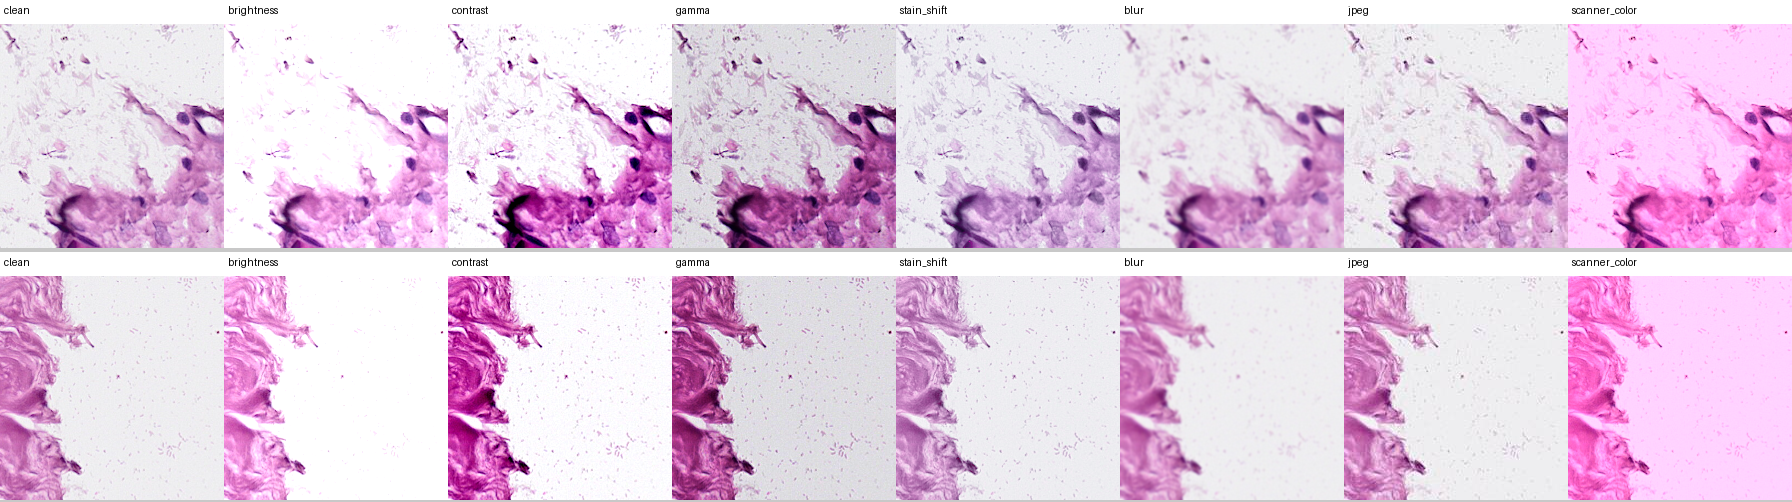
\includegraphics[width=\textwidth]{figures/perturbation_suite_example.png}
\caption{Two representative IDC patches (rows) under the full calibrated perturbation suite (columns), each perturbation individually tuned to mean SSIM$\approx$0.90 against the clean image (stain\_shift excluded from SSIM-matching by design). Morphology is visibly preserved throughout.}
\label{fig:perturbation_examples}
\end{figure}

\subsection{Gene-Program Flip Rate (GPFR)}
Five gene programs (immune activation, proliferation, hypoxia, stromal/ECM, angiogenesis) are scored from predicted expression via their MSigDB Hallmark \citep{msigdb_hallmark} gene sets, using log1p-normalized mean expression across each program's available genes; predicted expression is clipped to $\ge0$ before the log1p, since Ridge predictions for low-expression genes routinely go slightly negative. This clipping creates a dead zone for already-negative predictions -- a perturbation that pushes a clipped prediction further negative produces no score change for that gene -- which damps GPFR by an amount that depends on how often predictions are clipped, itself encoder-dependent since UNI's heavier shrinkage pulls predictions toward the positive training mean and clips less often (Section~\ref{sec:limitations}). Supplementary Table~S5 reports how many of each Hallmark set's genes are present on IDC's targeted panel: coverage ranges from 1.8\% (\texttt{proliferation}, 6 of 327 genes) to 13.9\% (\texttt{angiogenesis}, 5 of 36), and \texttt{angiogenesis}'s genes overlap substantially with other programs' (4 of its 5 genes also belong to \texttt{stromal\_ecm} or \texttt{hypoxia}). We use ``program'' throughout for consistency with Hallmark nomenclature rather than to claim comprehensive pathway coverage (Section~\ref{sec:limitations}).

For clean score $c_i$ and perturbed score $p_i$ of held-out sample $i$, with $\sigma_c$ the cohort's own standard deviation of clean scores:
\begin{equation}
z_i = \frac{|p_i - c_i|}{\sigma_c + \epsilon}, \qquad \text{flipped}_i = \mathbb{1}[z_i > z_{\text{thresh}}], \qquad \text{GPFR} = \frac{1}{N}\sum_i \text{flipped}_i
\end{equation}
with $z_{\text{thresh}}=1.0$ and $\epsilon=10^{-8}$. GPFR is an instantiation of the established decision-flip-rate family used to measure output instability under perturbation in clinical ML \citep{decisionflip_2603, decisionflip_2606}, applied here to a continuous, Hallmark-aggregated program score rather than a discrete classifier label or LLM answer. The per-sample-relative threshold is used rather than a single global absolute threshold because raw program-score magnitudes are not comparable across gene panels of different sizes; ``flipped'' is therefore defined relative to each cohort's own natural score spread. $z_{\text{thresh}}=1.0$ is a conventional, interpretable choice rather than one derived from a formal power analysis; Section~\ref{sec:results} reports a sensitivity sweep across $z_{\text{thresh}}\in\{0.5,0.75,1.0,1.5,2.0\}$.

\subsection{Statistical testing}
Held-out patches from the same slide are not independent draws, since they share slide-level staining, scanning, and tumor-composition variation. A bootstrap that resamples individual patches would treat the number of patches, not the number of slides (4, for IDC), as the effective sample size, understating the true variance of GPFR. For every (perturbation, program) pair, we therefore resample \emph{slides} with replacement 2{,}000 times (pooling every patch from each drawn slide) rather than resampling patches directly, recomputing GPFR each time, to obtain a 95\% bootstrap CI and a one-sided bootstrap $p$-value (the fraction of resampled GPFR values $\le 0$, testing against the boundary null of ``no sample ever flips''). A permutation-based null (shuffling the perturbed-score array relative to clean scores) is not appropriate for this statistic: because GPFR compares $|p_i - c_i|$ against the cohort's own between-sample spread, a full shuffle replaces $p_i$ with an unrelated sample's score from that same wide distribution, which is always noisier than correctly-paired data regardless of whether a real effect exists (verified with a synthetic, directly-constructed $\text{GPFR}=0.5$ effect, for which this null returned $p\approx1.0$). $p$-values across all 35 (perturbation, program) combinations per encoder are corrected via Benjamini-Hochberg FDR.

With only 4 slides, the cluster bootstrap's resampling distribution is itself coarse: at most $4^4=256$ distinct slide-draw outcomes are possible, so the one-sided $p$-value is quantized (6--9 distinct values across the 35 tests per encoder) and several $q$-values sit at the same BH-adjusted floor ($0.000583$ for CONCH, $0.000648$ for UNI). A percentile CI built from the same 2{,}000 resamples can therefore have a lower bound that rounds to $0.000$ even for a row whose $q$-value clears FDR$<$0.05, since the one-sided $p$-value and the two-sided percentile interval are different constructions from the same draws. Supplementary Tables~S1--S2 therefore star a row only when the CI itself excludes 0.000 in addition to clearing FDR$<$0.05, so the star is never contradicted by the interval printed beside it.

\subsection{Baseline predictors}
A held-out Pearson $r$ or $R^2$ is only informative relative to a floor. We fit two floor baselines on the identical IDC and COAD train/held-out splits (seed 42): (1) \texttt{training-mean}, which predicts every held-out patch's expression as the training set's per-gene mean; and (2) \texttt{total-counts-linear}, a per-gene linear regression from a single feature, the patch's own raw total panel counts. We report $R^2$ rather than Pearson $r$ for this comparison because $r$ is undefined for \texttt{training-mean}'s constant prediction.

\section*{Data Availability}
Patch and expression data are from HEST-Bench \citep{hest1k_2024} (CC BY-NC-SA 4.0); the IDC and COAD samples used here originate from publicly released 10x Genomics Xenium breast and colorectal cancer datasets respectively. Hallmark gene sets are retrieved from Enrichr's public MSigDB\_Hallmark\_2020 mirror. All results files underlying every table and figure in this paper, and the perturbation-calibration configuration, are available at \url{https://github.com/AbdelrahmanAboegela/fragile-foundations}.

\section*{Code Availability}
All analysis code (perturbation implementations, calibration, statistical testing, table/figure generation) is available at \url{https://github.com/AbdelrahmanAboegela/fragile-foundations}. CONCH and UNI checkpoints are obtained from their respective gated HuggingFace repositories under each model's own license terms and used strictly as frozen feature extractors.

\section*{Author Contributions}
A.A.A. conceived the study, designed and implemented the analysis pipeline, performed all experiments and statistical analyses, and wrote the manuscript.

\section*{Funding}
This research received no external funding.

\section*{Competing Interests}
The author declares no competing interests.

\section*{Supplementary Information}
Supplementary Information accompanies this paper.

\bibliographystyle{plainnat}
\bibliography{references}

\end{document}
